\clearpage

\subsection{Opaque without Survivability}\label{heuristic_Opaque_Survivability}
\begin{tcolorbox}	
\begin{tabular}{p{2.75cm} p{0.2cm} p{10.5cm}} 	
\textbf{Student Name}  &:& Tiago Esteves    (October 03, 2017 - )\\
\textbf{Goal}          &:& Implement the Heuristic model for the opaque transport mode without survivability.
\end{tabular}
\end{tcolorbox}

\subsubsection{Model description}

In an initial phase we will have two aspects to fulfill. The first one is to define the ODU0, ODU1, ODU2, ODU3 and ODU4 matrices, and the second one passes through the design of the network in question.
After this phase is completed, we then apply the algorithms created. first the "joinTrafficMatrices" then the "logicalTopology" and finally the "Grooming".
At the end, the algorithm "CostReport" will be applied to obtain the CAPEX result for the network in question.


\subsubsection{Result description}

We already have all the necessary formulas to obtain the CAPEX value for the reference network \ref{Reference_Network_Topology}. As described in the subsection of network traffic \ref{Reference_Network_Traffic}, we have three values of network traffic (low, medium and high traffic) so we have to obtain three different CAPEX.\\

\textbf{Low Traffic Scenario:}\\

Following all the steps mentioned in the previous subsection and using all the data referring to this scenario the obtained result can be consulted in the following table \ref{heuristicopaque_surv_ref_low}.

\begin{figure}[h!]
\centering
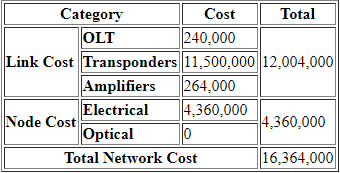
\includegraphics[width=9cm]{sdf/heuristic/figures/heuristic_opaque_surv_ref_low}
\caption{The network cost using Net2Plan.}
\label{heuristicopaque_surv_ref_low}
\end{figure}


\textbf{Medium Traffic Scenario:}\\


\textbf{High Traffic Scenario:}\\

Following all the steps mentioned in the previous subsection and using all the data referring to this scenario the obtained result can be consulted in the following table \ref{heuristicopaque_surv_ref_high}.

\begin{figure}[h!]
\centering
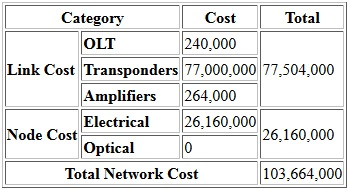
\includegraphics[width=9cm]{sdf/heuristic/figures/heuristic_opaque_surv_ref_high}
\caption{The network cost using Net2Plan.}
\label{heuristicopaque_surv_ref_high}
\end{figure}
